\documentclass[10pt,a4paper]{article}
\usepackage[utf8x]{inputenc}
\usepackage[T1]{fontenc}
%\usepackage{stringenc} % for grffile
\usepackage{ucs}
\usepackage{amsthm} %numéroter les questions
\usepackage[english]{babel}
\usepackage{datetime}
\usepackage{xspace} % typographie IN
\usepackage{hyperref}% hyperliens
\usepackage[all]{hypcap} %lien pointe en haut des figures
\usepackage[english]{varioref} %voir x p y
\usepackage{fancyhdr}% en têtes
%\input cyracc.def
\usepackage[]{graphicx} %include pictures
%\usepackage[encoding,inputencoding=utf8,filenameencoding=utf8]{grffile}
%\usepackage[extendedchars,inputencoding=latin1,filenameencoding=latin1]{grffile}
\usepackage[siunitx ]{circuitikz}
\usepackage{gnuplottex}
\usepackage{ifthen}
\graphicspath{{./figures/}}
%\usepackage{array}
\usepackage{amsmath}
\usepackage[]{xcolor}
\usepackage{tikz}
\usepackage{tikz-timing}
\usetikzlibrary{scopes}
\usetikzlibrary{backgrounds}
\usepackage{listings}
\usepackage{enumitem}
\usepackage[top=1 in, bottom=1 in, left=1.3 in, right=1 in]{geometry} % Yeah, that's bad to play with margins
\usepackage[]{pdfpages}
\usepackage{pdflscape}
\usepackage[]{attachfile}
%\usepackage{colortbl}
%\usepackage{multirow}
\usepackage{booktabs}
\usepackage{makecell}
\usepackage[ ]{subfig}
%\usepackage{rotating}
\usepackage{upgreek}
\usepackage[normalem]{ulem}
\usepackage{url}
\makeatletter
\g@addto@macro{\UrlBreaks}{\UrlOrds}
\makeatother

\newdateformat{mydate}{2020--2021}%hack pour remplacer \THEYEAR

%cyr
%\newcommand\textcyr[1]{{\fontencoding{OT2}\fontfamily{wncyr}\selectfont #1}}
\renewcommand{\marginpar}[1]{} %surcharge pour /marginpar

\newboolean{corrige}
%\setboolean{corrige}{true}%corrigé
\setboolean{corrige}{false}% pas de corrigé

\newboolean{annexes}
%\setboolean{annexes}{true}%annexes
\setboolean{annexes}{false}% pas de annexes

\newboolean{mos}
%\setboolean{mos}{true}%annexes
\setboolean{mos}{false}% pas de annexes

\usepackage{aeguill} %guillemets

%% fancy header & foot
\pagestyle{fancy}
\lhead{[ELEC-H-410] Real-Time systems Lab n° 0: PSoC and logic analyzers}
\rhead{\mydate\today\\ page \thepage}
\chead{\ifthenelse{\boolean{corrige}}{Corrigé}{}}
\cfoot{}
%%

\pdfinfo{
    /Author (BEAMS)
    /Title (Lab n° 0 ELEC-H-410, RTOS)
    /ModDate (D:\pdfdate)
}

\hypersetup{
    pdftitle={Lab n° 0 [ELEC-H-410] Real-Time systems},
    pdfauthor={BEAMS},
    pdfsubject={PSoC and logic analyzers}
}

\theoremstyle{definition}% questions pas en italique
\newtheorem{E}{\color{blue}Exercise}[] % numéroter les questions [section] ou non []

\newcommand{\reponse}[1]{% pour intégrer une réponse : \reponse{texte} : sera inclus si \boolean{corrige}
	\ifthenelse {\boolean{corrige}} {\paragraph{Réponse :} #1} {}
 }

\newcommand{\addcontentslinenono}[4]{\addtocontents{#1}{\protect\contentsline{#2}{#3}{#4}{}}}

\newcommand{\on}[1]{\operatorname{#1}}

\newcommand{\reg}[1]{\texttt{reg#1}}

\newcommand{\rtos}{FreeRTOS}

\newcommand{\kw}[1]{\texttt{#1}}

\setlength{\parskip}{1ex plus .5ex minus .5ex} % espacement entre paragraphes
\setlength{\parindent}{0 ex plus 0ex minus 0 ex} % retrait en début de §

\def\labelitemi{--}
\setlist{parsep=0pt,itemsep=0pt,style=standard,leftmargin=\parindent, align=left} % pas d'espace prohibitif entre les items
\setlist{nolistsep}

\newcolumntype{C}[1]{>{\centering\let\newline\\\arraybackslash\hspace{0pt}}m{#1}}

%\setlength{\tabcolsep}{0pt} %no extra space in cells to keep constant tabular width

\date{\vspace{-1cm}\mydate\today}
\title{\vspace{-2cm} Lab n° 0\\ Real-Time systems [ELEC-H-410]\\ Introduction to PSoC microcontrollers and logic analyzers~\ifthenelse{\boolean{corrige}}{~\\Corrigé}{}}

%\author{\vspace{-1cm}}%\textsc{Yannick Allard}}


\lstdefinestyle{customasm}{
    % belowcaptionskip=1\baselineskip,
    % frame=L,
    % xleftmargin=\parindent,
    language=[x86masm]Assembler,
    basicstyle=\footnotesize\ttfamily,
    commentstyle=\itshape\color{purple!40!black},
    comment=[l]//,
}
\lstdefinestyle{customc}{
    belowcaptionskip=1\baselineskip,
    breaklines=true,
    frame=L,
    xleftmargin=\parindent,
    language=C,
    showstringspaces=false,
    basicstyle=\footnotesize\ttfamily,
    keywordstyle=\bfseries\color{green!40!black},
    commentstyle=\itshape\color{purple!40!black},
    identifierstyle=\color{blue},
    stringstyle=\color{orange},
}
\lstset{escapechar=@,style=customc}

\begin{document}

    % Introduce a new counter for counting the nodes needed for circling
    \newcounter{nodecount}
    % Command for making a new node and naming it according to the nodecount counter
    \newcommand\tabnode[1]{\addtocounter{nodecount}{1} \tikz \node (\arabic{nodecount}) {#1};}
    
    % Some options common to all the nodes and paths
    \tikzstyle{every picture}+=[remember picture,baseline]
    \tikzstyle{every node}+=[inner sep=0pt,anchor=base]
    \tikzstyle{every path}+=[thick, rounded corners]
    % for tikz pict
    
    \maketitle
    In order  for you to work remotely, we changed this year project into a game. The game simulates a pandemic situation, very much like the one we are seeing right now. As you have seen, real-time response is a critical component of handling a pandemic efficiently. 

It is by no means our intention to take the current epidemic lightly. However, we thought that this project assignment would allow to lighten the mood a little, as everyone's morale will also be taking a serious hit during this period of confinement. Keep your spirits high and make sure you give your courses your best (all of them, not just this one). We will need talented and bright engineers in the aftermath of this crisis.  

To play this game, you don't need any equipment other than the PSOC itself.
The game is entirely coded inside one FreeRTOS task (\textit{gameTask}).
It sends "events" and we ask you to make a code that will automatically respond to those "events".\\
Depending on your response time you will increase or not some variables.

\subsection*{Useful documentation:}
\begin{itemize}
    \item Official \rtos~ documentation: \url{https://www.freertos.org/Documentation/RTOS_book.html}
    \item Getting Started with PSoC 5LP: \url{https://www.cypress.com/file/41436/download}
    \item Video example on how to use the PSoC: \url{https://www.cypress.com/video-library/PSoC}
    \item The extension board schematics: \texttt{Extension\_PSoC.pdf}
		\item Getting started with the Logic Analyzer: \url{https://learn.sparkfun.com/tutorials/using-the-usb-logic-analyzer-with-sigrok-pulseview}
\end{itemize}

    \newpage 
		
\section{Introduction to the PSoC microcontroller}

The first part of the lab is to help you familiarize yourself with the PSoC microcontroller. For students who have had the course ELEC-H-310, this will mainly be a reminder of the course's labs. 

You should start by installing the PSoC Creator IDE, as explained in Appendix~\ref{app:software_psoc}. If you are not confident with C programming, read \texttt{C\_language\_for\_uC.pdf}.

In the following subsections, you will learn how to instantiate and use some basic hardware components of the PSoC microcontroller: 
\begin{itemize}
	\item GPIOs (including LEDs and pushbuttons of the extension board); 
	\item the LCD screen; 
	\item the keyboard. 
\end{itemize}
You can always refer to refer to the PSoC tutorials (\url{www.cypress.com/psoc101}) or the datasheet of the hardware elements (these can be found by double-clicking on a component in the \texttt{TopDesign.cysch} file, and clicking on the button \texttt{Datasheet}). 




\subsection{General purpose input-output (GPIO)}

GPIOs are the most basic hardware elements, allowing to provide input commands to the microcontroller and receive output signals from the microcontroller. You can find tutorials of how to use GPIOs on the following website: 
\begin{itemize}
	\item \url{www.cypress.com/psoc101}, Lesson 1: ``1. Software Output Pins''
	\item \url{www.cypress.com/psoc101}, Lesson 2: ``2. Software Input Pins''
\end{itemize}
The following exercise will help you to interface two sort of IOs~: push-buttons and LEDs. The following (partial) list of functions are useful for using the GPIOs: 
\begin{itemize}
		\item \kw{gpioName\_Read()}: Read a GPIO value; 
		\item \kw{gpioName\_Write(value)}: Write a binary value to a GPIO;   
		\item \kw{CyDelay()}: use this function to put the microcontroller to sleep for a certain amount of milliseconds between two iterations of the for loop. 
\end{itemize}

\E{
\label{ex:1}
Open the \kw{Lab0} project. In this project, the different hardware components of the extension board have already been instantiated. 
\begin{itemize}
	\item Identify which hardware elements have been instantiated in the \texttt{TopDesign.cysch} file. You can have the details of a hardware component by double-clicking on it. 
	\item In the \texttt{Lab0.cydwr} file, the instantiated hardware elements have been associated with the pins of the PSoC microcontroller. Can you match the pin numbers of the PSoC with the hardware elements of the extension board by using the electrical schematics in Appendix~\ref{app:extension_psoc}? 
	\item Now write the code in the \texttt{main.c} file such that the LEDs D1-D4 turns on when the corresponding button SW1-SW4 is pushed, and turns off when this button is released. 
	\item Build, compile and load it on the PSoC board, then check its behavior (the shortcut buttons to build, compile and program the PSoC are located on the ribbon on the top left of the PSoC IDE). 
\end{itemize}
It is important to note that, in general, microcontroller are not designed to deliver high currents. If we were using high-brightness LEDs, we would need to use \textit{buffer} circuits (such as the \texttt{74ACT244}) to provide larger currents. 
}
{}






\subsection{LCD screen}

The LCD screen is a particular output that allows you to write characters on the 16-characters LCD screen, located on the extension board. By examining Appendix~\ref{app:extension_psoc}, you will notice that the LCD requires 7 output ports from the microcontroller. On the left side of the LCD screen, there is a potentiometer that allows you to control the contrast of the LCD screen. The 8 first characters of the LCD screen are defined to be row~0, the 8 last characters of the LCD screen are defined to be row~1. The exact mapping of the rows and columns of the LCD screen are shown in Figure~\ref{fig:lcd_screen}. 
\begin{figure}[h]
	\centering
	\includegraphics[width=4in]{lcd_screen.png}
	\caption{Row and column mapping of the LCD screen. }
	\label{fig:lcd_screen}
\end{figure}
The following (partial) list of functions are useful for using the LCD screen: 
\begin{itemize}
		\item \kw{LCD\_Init()}: to initialize the LCD; 
		\item \kw{LCD\_ClearDisplay()}: to clear the LCD display; 
		\item \kw{LCD\_Position()}: to control the cursor position of the LCD display; 
		\item \kw{LCD\_PrintString()}: to print a string of characters; 
		\item \kw{LCD\_PrintNumber()}: to print the decimal value of a 16-bit value; 
		\item \kw{LCD\_PrintInt8()}: to print a two-ASCII-character hex representation of the 8-bit value; 
		\item \kw{LCD\_PrintInt16()}: to print a four-ASCII-character hex representation of the 16-bit value; 
		\item \kw{LCD\_PutChar()}: to print \texttt{char} value; 
\end{itemize}

\E{
\label{ex:2}
Open the \kw{Lab0} project, which has already instantiated the LCD screen. Write a code such that counts the number of times that SW2 is pressed, and prints this value on the LCD screen under the format ``SW2 count: 8'' (where 8 should be replaced with the number of times SW2 is pressed). 
{}







\subsection{Keyboard}

A small $4\times 3$ keyboard is provided, that can be connected directly to the bottom of the extension board\footnote{there are 8 pins to the bottom of the extension board to allow for $4\times 4$ keyboards. Please use the seven leftmost pins for a $4\times 3$ keyboard. }. 
\begin{figure}[h]
	\centering
	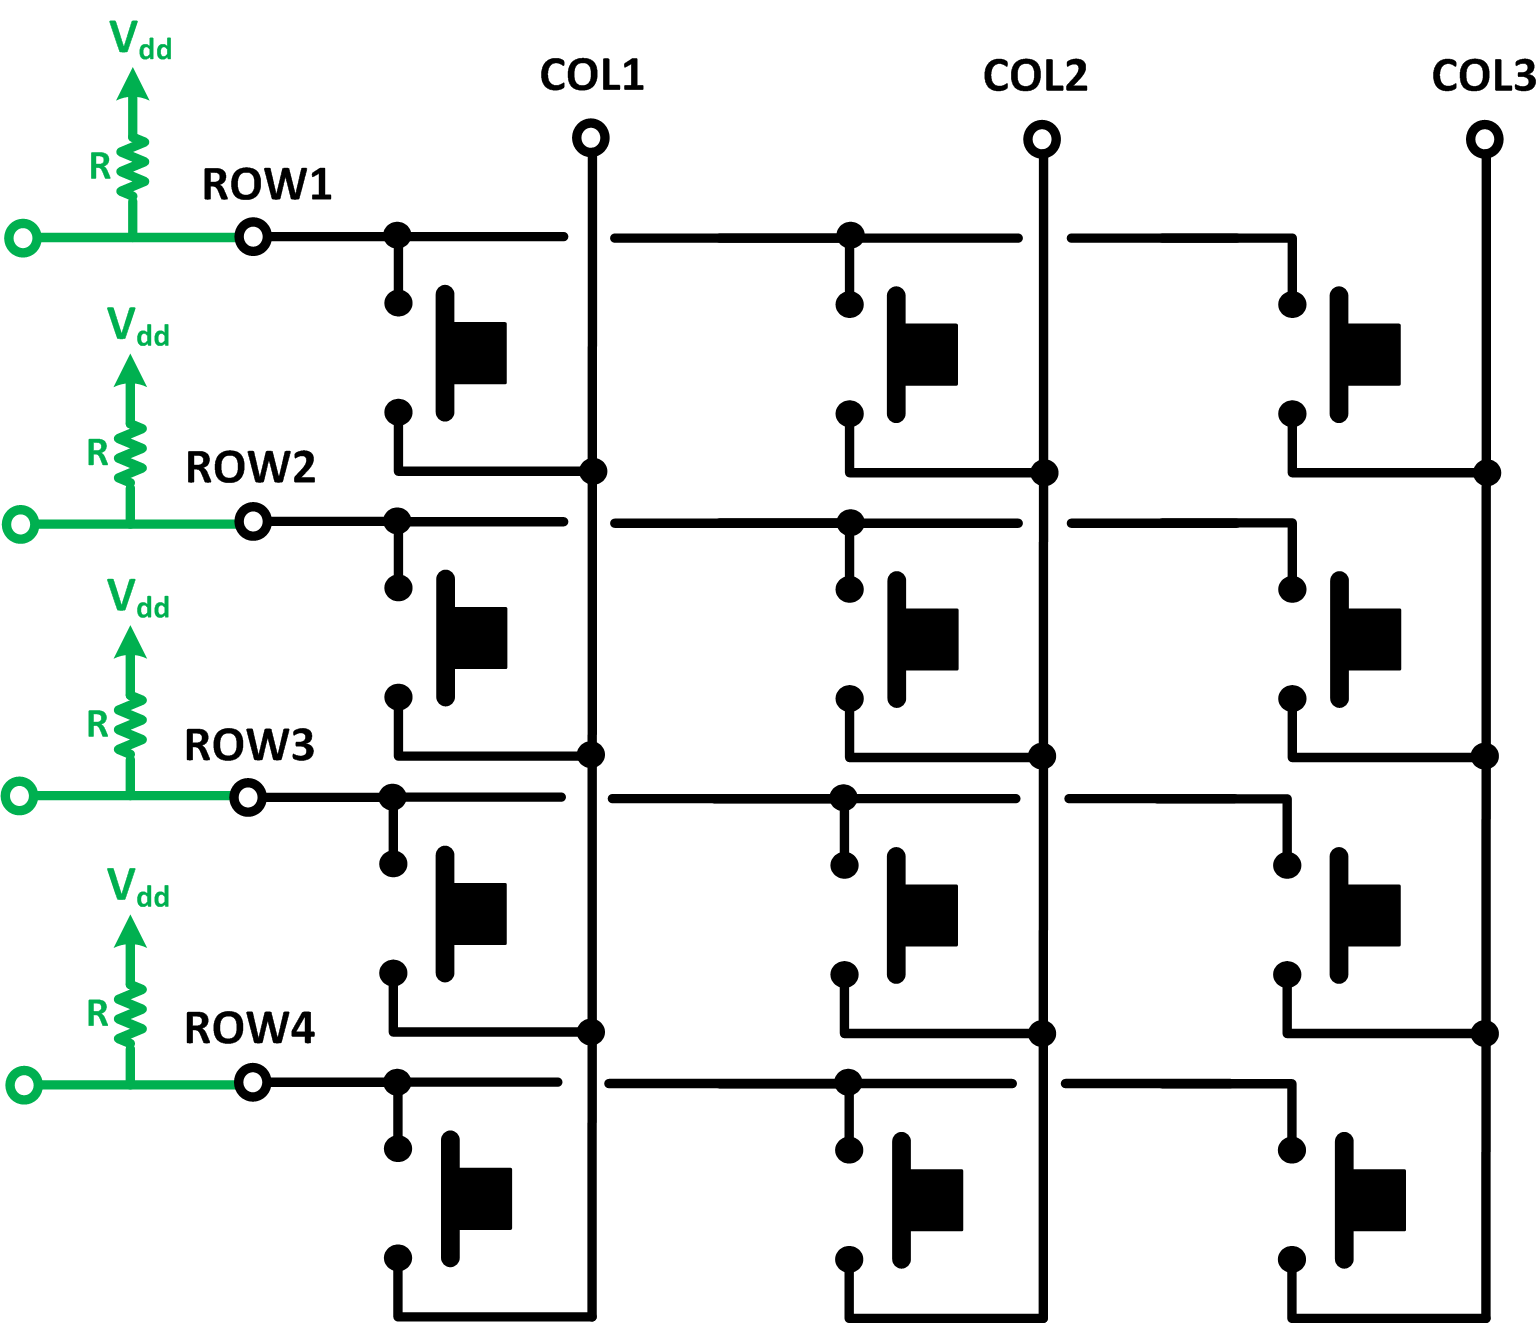
\includegraphics[width=2.5in]{keyboard.png}
	\caption{Electronic circuit of a $4\times 3$ keyboard. The green part represents the resistive pull-ups inputs of the PSoC board. }
	\label{fig:keyboard}
\end{figure}
A library has already been created and included in the project, and the keyboard has been instantiated in the \texttt{TopDesign.cysch} file. You can use the following function that are included in the library: 
\begin{itemize}
		\item \texttt{keyboard\_Start()} to initialize the keyboard; 
		\item \texttt{keyboard\_Scan()} to scan the keyboard. This will return the value that is pressed as a \texttt{uint8\_t}, and it will return the value \texttt{z} if no key is pressed. 
\end{itemize}

\E{
\label{ex:3}
Now write a code that prints successive pressed keys on the LCD screen. Your code should scan the keyboard every 50~ms. Note that if the keyboard is pressed only once, the value should be printed only once on the LCD screen. 
{}








		
\section{Introduction to the logic analyzer}

The second part of the lab is to help you familiarize yourself with the logic analyzer. 

You should start by installing the logic analyzer software, as explained in Appendix~\ref{app:software_logic_analyzer}. You can connect the female-to-female cables to the logic analyzer inputs, and male-to-male pin headers at the end of each cable (feel free to detach the cables and to snap the male-to-male pin headers to the amount you prefer). 

In the following subsections, you will learn how to operate the logic analyzer: 
\begin{itemize}
	\item running the logic analyzer manually; 
	\item using the logic analyzer trigger. 
\end{itemize}
You can always refer to the logic analyzer tutorial (\url{https://learn.sparkfun.com/tutorials/using-the-usb-logic-analyzer-with-sigrok-pulseview}). 




\subsection{Running the logic analyzer manually}

We will use the logic analyzer to measure the execution time of parts of our code. The code needs to be instrumented to make internal signals from the microcontroller visible from the outside. 

\E{
\label{ex:4}
In this exercise, we will measure the period at which a GPIO is toggled. 
\begin{itemize}
	\item Using the \texttt{CyDelay} function, write a code to toggle the first GPIO on jumper J1 of the extension board at a frequency of 20~Hz. There is no need to use a hardware timer for this exercise; 
	\item Connect the analyzer to the extension board as shown in Figure~\ref{fig:analyserConnection}. 
	\item Use the \texttt{PulseView} software to measure the period with which the GPIO is toggled. 
\end{itemize}
}
{}

\begin{figure}[h]
	\centering
	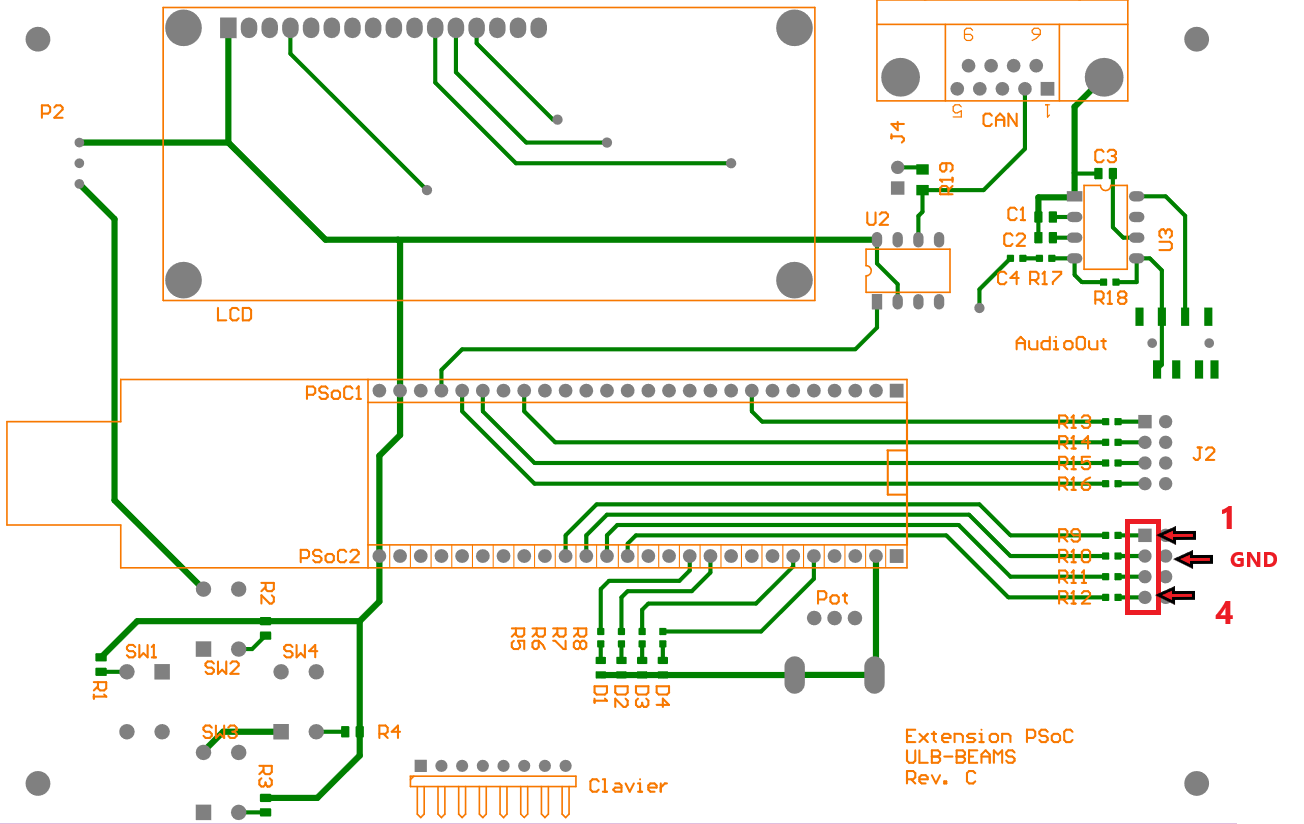
\includegraphics[width=4in]{analyserConnection.png}
	\caption{Where to connect the logic analyzer to the extension board. }
	\label{fig:analyserConnection}
\end{figure}




\subsection{Using the logic analyzer trigger}

A trigger can be used to automate the acquisition of the logic analyzer. You can select a trigger by selecting the channel to trigger on (e.g. D3) and selecting the required trigger (e.g. rising edge). 

It is also possible to trigger the acquisition based on multiple channels, you just need to specify the trigger condition for each channel (e.g. trigger when D1 is high and D2 has a rising edge). 

\E{
\label{ex:5}
In this exercise, we will trigger the logic analyzer when SW4 is pressed. 
\begin{itemize}
	\item Extend your previous code such that the second GPIO of jumper J1 becomes high when SW4 is pressed, and becomes low when SW4 is released; 
	\item Specify a trigger condition such that the logic analyzer acquisition is triggered when SW4 is pressed. 
	\item Extend your previous code and trigger conditions such that the acquisition is triggered when SW3 is high and SW4 is pressed. 
\end{itemize}
}
{}










		
    \vfill
    \footnotesize{Found an error? Let us know: \url{https://github.com/BEAMS-EE/ELECH410/issues}}
    
		\appendix
    \newpage 
\section{PSoC software}
\label{app:software_psoc}

To program the PSoC microcontroller, you need to install the PSoC Creator software suite. You can download this software on the following website: \\
\url{https://www.cypress.com/products/psoc-creator-integrated-design-environment-ide}. The software is quite large, so it might take a while to download. You can then install the software suite. \\
You should also download the CY8CKIT-059 Kit setup on \url{https://www.cypress.com/file/416376/download} (you might need to create an account to download this file). Once downloaded, you should execute the downloaded file to install the CY8CKIT-059 Kit. 
\\
\\
When launching the PSoC Creator IDE, it will usually ask you to register. You can ignore this by selecting ``Register later''. When creating a new project, you need to specify which microcontroller you are using. In this project, we will use the ``CY8CKIT-059 (PSoC 5LP)''. Once your project is created, your project will be loaded as shown in Figure~\ref{fig:psoc_creator_ide}. 
\begin{figure}[h]
	\centering
	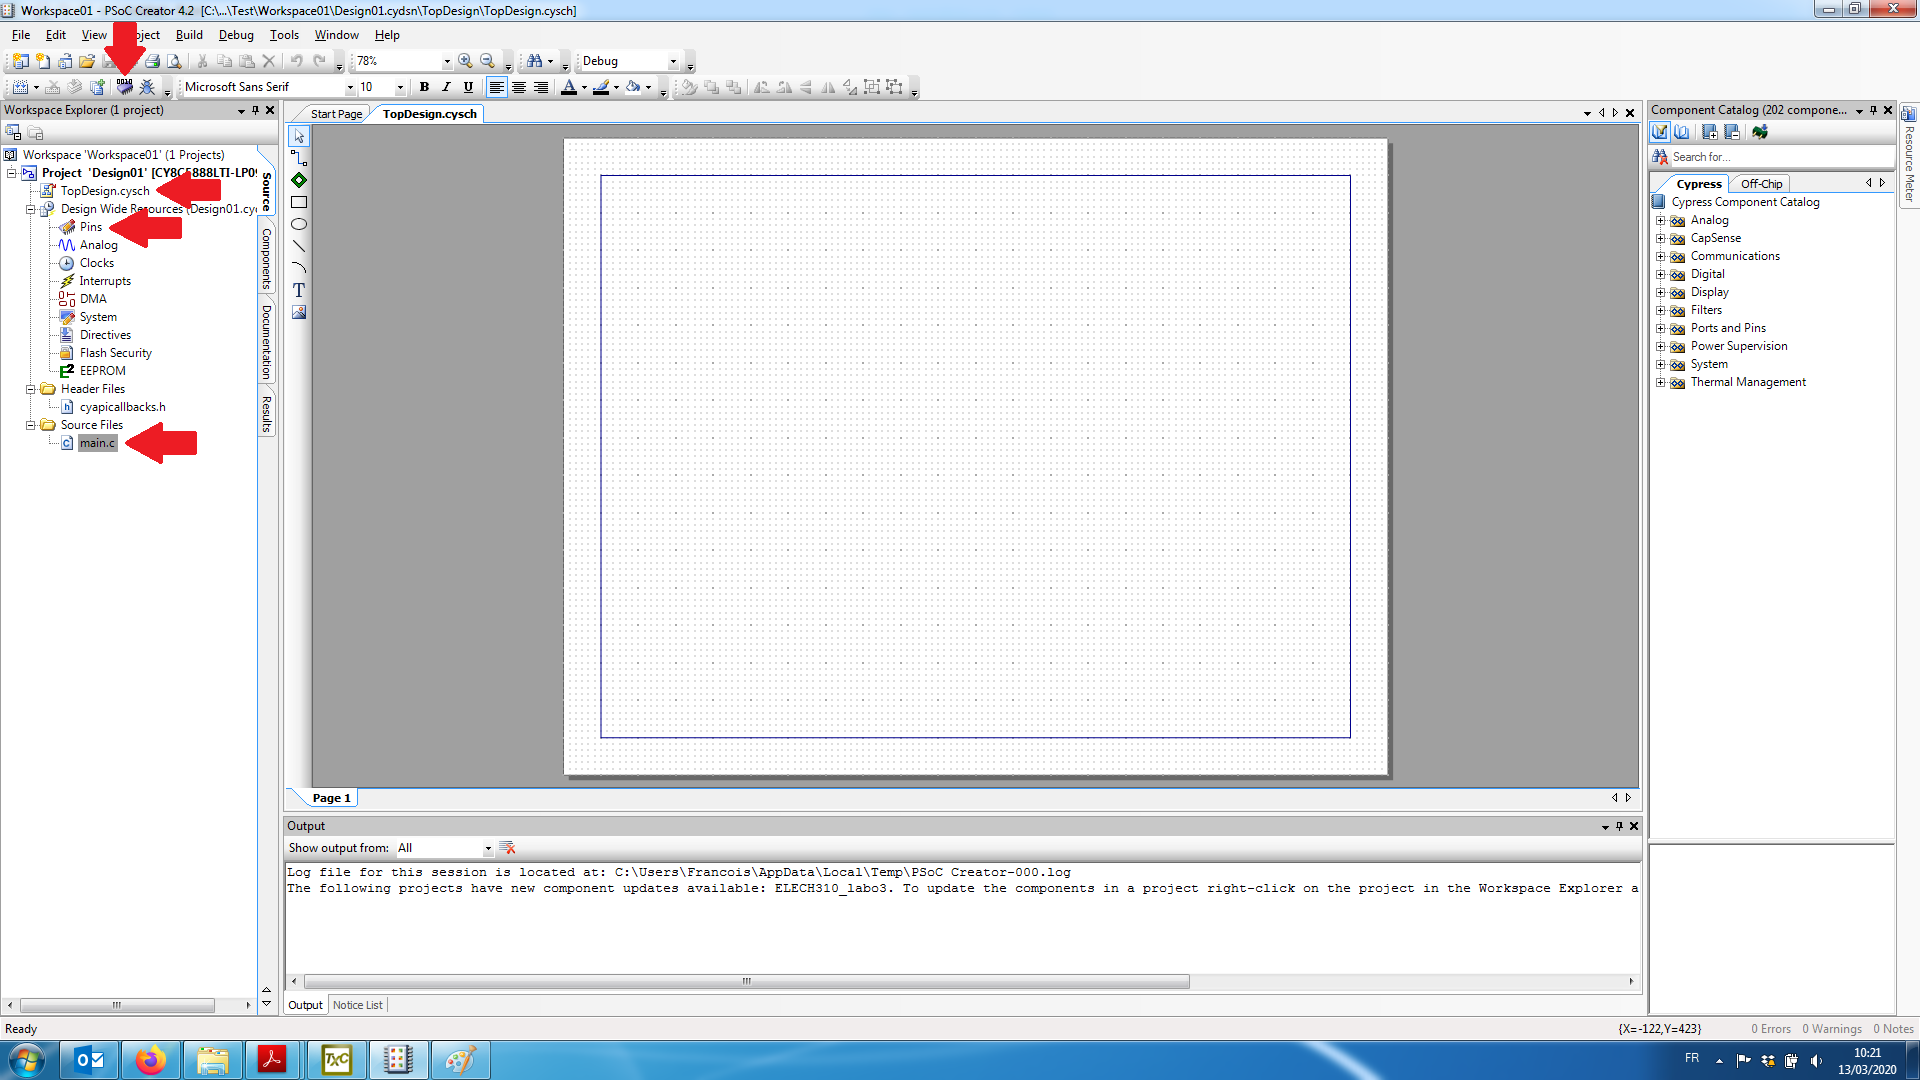
\includegraphics[width=5in]{psoc_creator_ide.png}
	\caption{PSoC Creater IDE. }
	\label{fig:psoc_creator_ide}
\end{figure}
\begin{figure}[h]
	\centering
	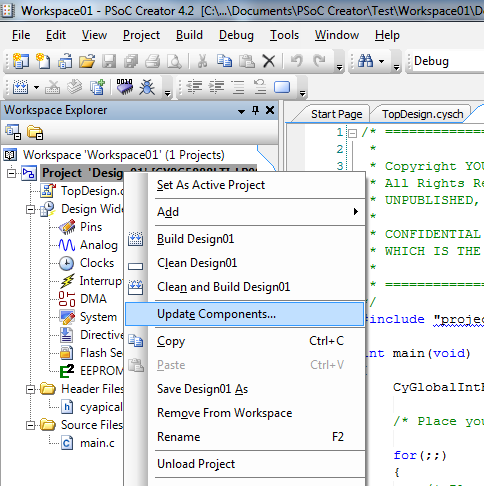
\includegraphics[width=2in]{update_components.png}
	\caption{How to update the PSoC firmware. }
	\label{fig:update_components}
\end{figure}

In this project, you will mainly be using three tabs of the IDE: 
\begin{itemize}
	\item \textbf{TopDesign.cysch: } In this window, you will instantiate all the hardware elements that you will use in the microcontroller, i.e. the GPIOs, the ADC, the DAC, the PWM, the LCD screen, etc. 
	\item \textbf{Pins: } This window will help you to associate each hardware element you instantiated to an actual output pin of the PSoC board. The numbers of each pin is written on the PSoC board itself, and you can use the document \texttt{Extension\_PSoC.pdf} to see which pin of the PSoC board was connected to which input/output of the custom-designed extension board. One of the particularities of the PSoC board is that each hardware element can be connected to any pin. 
	\item \textbf{main.c: } In this window you will write the firmware, i.e. the actual program that will be executed on the microcontroller. The code mainly consists of a main function that contains an initialization code and an infinite for-loop. Your microcontroller will continuously execute the program that is written in the infinite for-loop until the microcontroller is turned off.  
\end{itemize}

To upload your program to the PSoC board, connect the PSoC programmer to your computer with the USB cable, and click the ``Program'' button. This will build, compile and upload your project to the microcontroller. Useful documentation can be found on the following websites: 
\begin{itemize}
	\item Getting Started with PSoC 5LP: \url{https://www.cypress.com/file/41436/download}
	\item Tutorials for each hardware element of the PSoC: \url{www.cypress.com/psoc101}
  \item Video example on how to use the PSoC: \url{https://www.cypress.com/video-library/PSoC}
\end{itemize}
It is possible that the first time you try to upload a program to the PSoC board, you get an error message. This is because the firmware on the PSoC board needs to match the software version of PSoC Creator IDE. To solve this problem, right-click on the project and select ``Update components'' (see Figure~\ref{fig:update_components}. Then just follow the instructions with the default settings. 
		\newpage \section{Extension PSoC}
\label{app:extension_psoc}

The following pages contain the detailed schematics of the custom-made extension board for the PSoC device. 
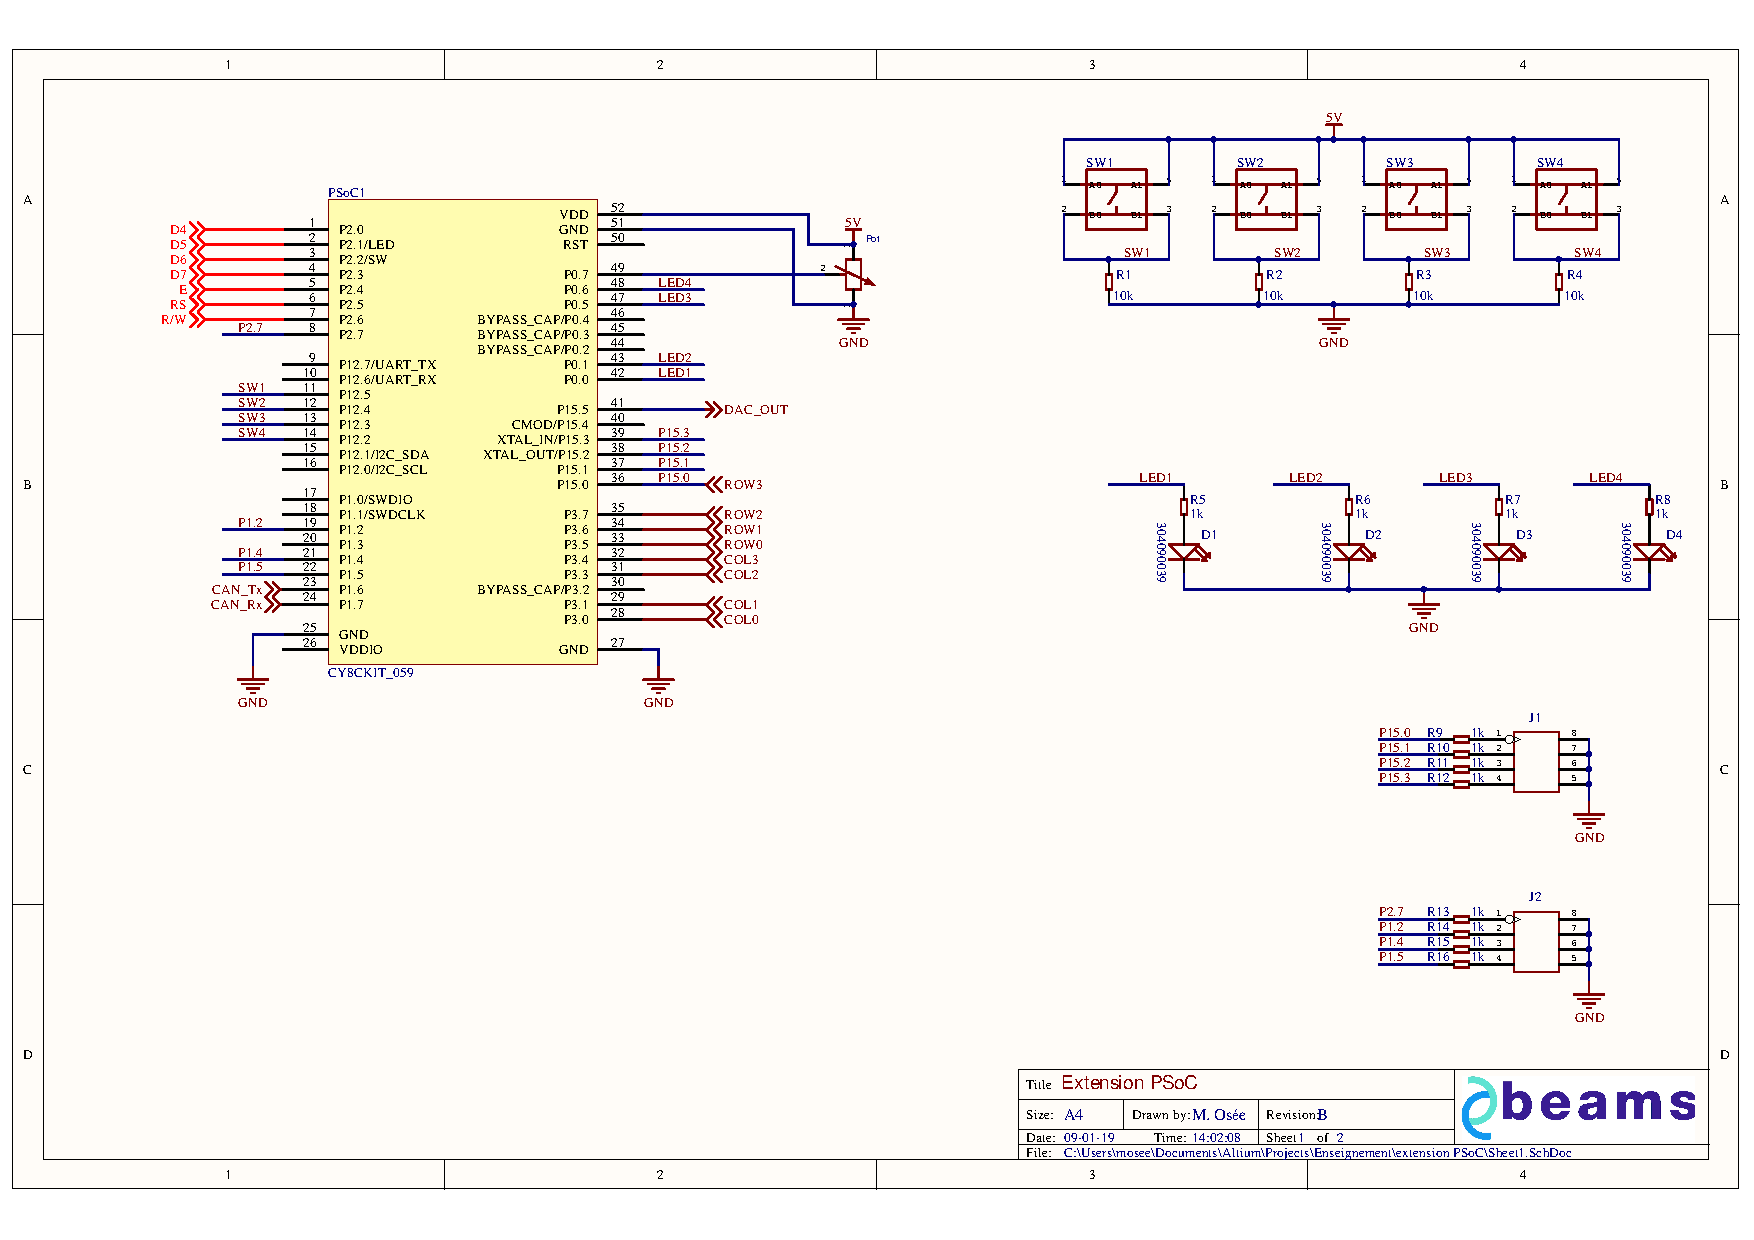
\includepdf[pages=-,angle=90]{figures/Extension_PSoC.pdf}
		\newpage 
\section{Logic Analyzer software}
\label{app:software_logic_analyzer}

To control and operate the logic analyzer, you must install the drivers for the logic analyzer and the \texttt{PulseView} software. All of these are available on \url{https://sigrok.org/wiki/Downloads}, where you need to download: 
\begin{itemize}
	\item \texttt{sigrok-cli}, which contains the drivers for the logic analyzers; 
	\item \texttt{PulseView}, which allows to operate the logic analyzers and visualize the data. 
\end{itemize}
Download and install both of these programs. 

Once both of these programs are installed, connect the logic analyzer to an USB port, and run \texttt{zadig.exe (sigrok-cli)}. Click on \texttt{Install Driver}. Once the drivers are installed, close the program. 

You can now run \texttt{PulseView}. If the logic analyzer is connected, it should be recognized by \texttt{PulseView} automatically (it should appear as ``Saleae Logic'' in the connected device). If it's not connected automatically, you should do the following: 
\begin{itemize}
	\item Click on the small arrow next to \texttt{Demo device} or \texttt{<No Device>}; 
	\item Click on \texttt{Connect to Device}; 
	\item In the \texttt{Choose the driver} menu, select \texttt{fx2lafw (generic driver for FX2 based LAs)}; 
	\item Click \texttt{Scan for devices using the driver above}; 
	\item Select \texttt{Saleae Logic with 8 channels} and click \texttt{OK}. 
\end{itemize}
You should see the 8 channels D0-D7, corresponding to the 8 logic channels of the logic analyzer. 



\end{document}




